Nesse problema, utilizamos o fato de que temos um Hamiltoniano mais simples, tal como:

\begin{equation}
V_{AB} = g\left( \sigma_{+}^{A} \sigma_{-}^{B} + \sigma_{+}^{B} \sigma_{-}^{A} \right) 
\end{equation}

Esse Hamiltoniano somente afeta o sistema quando temos um estado específico, advindo de combinações de estados dos dois sistemas interagentes. Pois ele aumenta o nível de um sistema enquanto abaixa o outro. Assim, quando os dois sistemas $A$ e $B$ estiverem no nível mais energético, eles apenas mudarão por uma fase. Quando estiverem no nível menos energético, o mesmo ocorre. Somente quando ambos estiverem com estados opostos , ou \textit{spins} opostos, teremos uma interação mais complicada. No espaço produto dos sistemas, o operador evolução será dado por:

\begin{equation}
U = \left[\begin{matrix}e^{- i \Omega t} & 0 & 0 & 0\\0 & \cos{\left (g t \right )} & - i \sin{\left (g t \right )} & 0\\0 & - i \sin{\left (g t \right )} & \cos{\left (g t \right )} & 0\\0 & 0 & 0 & e^{i \Omega t}\end{matrix}\right]
\end{equation}

Assim, a probabilidade de troca de calor somente existe quando temos o estado em que os sistemas interagentes estão em situações opostas. Com a construção dos produtos tensoriais, podemos ilustrar, através de um cálculo numérico, o que ocorre quando variamos a situação em termos de condição inicial do sistema $B$. Como o sistema $A$ carrega informação para o sistema $C$, seu valor final de expectativa de energia será dependente da temperatura de $B$. Podemos observar isso na Figura \ref{energias_bb_2}.

\begin{figure}[!h]
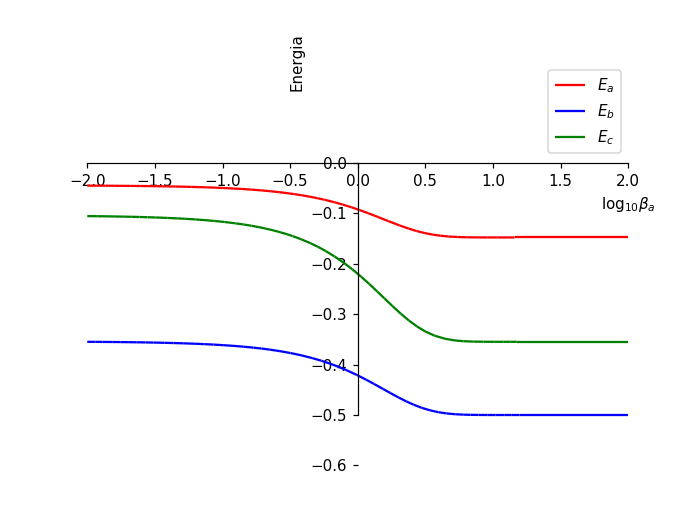
\includegraphics[scale=.45]{Content/energias_bb_2.png}
\caption{Valores esperados das energias finais para os três sistemas. Os parâmetros escolhidos nos cálculos foram $\Omega=1$, $g=0.1$, $\tau=10$,$\beta_a=10^2$ e $\beta_c=10^{-2}$.}
\label{energias_bb_2}
\end{figure}